%Linea Para poder completar automaticamente las citas con el Sublime
%No hace el documento, se puede borrar esta linea si no se usa el Sublime
%------------------------------------------------------------------------------
 \newcommand{\NoBiblioMicro}[1]{
 \ifthenelse{\equal{#1}{verdadero}}{}{\bibliography{Referencias/base_bibliografica}}
 \NoBiblioMicro{verdadero}}
 %-----------------------------------------------------------------------------

%Formato (Nombre de capitulo largo o corto), nombre del capitulo, resumen y estilo de la
%Portada del Capitulo
%------------------------------------------------------------------------------
 
 %Formato en si, titulo en dos renglones
 \FormatoCapituloDosLineas
 
 %Nombre y etiquete para referir
 \chapter{Microfabricación de multisensores electroquímicos}\label{chap:Microfabricacion}

 %Para que no salga el numero de pagina en la portada del capitulo
 \thispagestyle{empty}
	
 %Resumen del Capitulo en Italica
 %\noindent\textit{En este capítulo se describen los resultados obtenidos durante en la fabricación de electrodos recubiertos con películas delgadas mesoporosas de SiO$_2$ o Si$_x$Zr$_{1-x}$O$_2$. Se analizan los diseños utilizados, los materiales empleados, las técnicas aplicadas y las caracterizaciones llevadas a cabo. Principalmente se evaluó el desempeño electroquímico de los electrodos por un lado, y la compatibilidad con las síntesis sol-gel por otro, de forma de compatibilizar los procesos \textit{top-down }con los \textit{bottom-up.}. Por último se presentan los resultados EQ  para sondas modelos (\fe, \ru\space y \fc)obtenidos con un prototipo de sensor compuestos por electrodos recubiertos con distintas películas.}\index{bottom-up@\textit{bottom-up}}\index{top-down@\textit{top-down}}
 
 
 %Indice de capitulo alineada al borde inferior de la pagina, nueva pagina
 \vfill
 \minitoc
 \newpage
 %-------------------------------------------------------------------------------

\section{Introducción}
	
	El diseño y desarrollo de un multisensor electroquímico selectivo, integrado y escalable basado en \pdm\space consta de dos bloques constructivos fundamentales: los electrodos y las películas delgadas mesoporosas. En el capítulo \ref{chap:Mesoporosos}, se discutió y analizó la elección de los materiales para conformar la película delgada mesoporososa con la cual se recubren los electrodos. En el capítulo \ref{chap:Electroquimica} se realizó un estudio profundo de las propiedades permeoselectivas, la capacidad de preconcentrar, excluir y sobre la estabilidad química de dichos recubrimientos sobre electrods de Au.

	La integración de los procesos \textit{bottom-up}, propios de procesos de síntesis químicas, y \textit{top-down}, aquellos usados en microfabricación, nunca es trivial. El sólo hecho de depositar soles con precursores de óxidos sobre oro, que resulten en películas delgadas homogéneas, bien adheridas, sin grietas ni fisuras, ya es un desafío, como se vió en el capítulo \ref{chap:Mesoporosos}. El objetivo, luego de desarrollar los métodos a bajas temperaturas para la síntesis de \pdm, de optimizar y estudiar su estructura, y de comprender los procesos de transporte a través de las películas, es poder depositar las \pdm\space sobre películas delgadas de oro con motivos arbitrarios en base a un diseño racionalizado y optimizado para usarlo como multisensores. 

	El depósito de soles sobre una superficie que tenga dos o más capas de distintos  materiales trae asociadas dificultades inherentes a las propiedades físicas y químicas de cada uno de ellas. Pueden diferir en el coeficiente de expansión térmica, en la química superficial, en la afinidad por el H$_2$O o solventes, etc.
	Es por ello que el diseño debe considerar los materiales que se usarán y sus propiedades, así como racionalizar la estructura de los electrodos considerando resistencia eléctrica, espesor de los electrodos y facilidad para la fabricación. También es fundamental tener en cuenta una serie de factores a la hora de imprimir las máscaras para los sensores. Principalmente, la resolución de línea que se puede obtener según el tipo de máscara, cantidad de electrodos de trabajo por sensor, calcular el área óptima para obtener señales aceptables, estimar resistencia eléctrica, distancias entre electrodos y demás parámetros.

	El material para los electrodos también se debe elegir cuidadosamente. Se trata de un compromiso entre tres factores: 1) compatibilidad con el óxido de las películas mesoporosas, 2) obtención de una respuesta electroquímica de calidad y, 3) facilidad para depositarlos y transferir los diseños por litografía.

	En esta parte del trabajo se priorizó generar diseños compactos, miniaturizar los electrodos y optimizarlos para obtener respuestas electroquímicas de buen desempeño. El oro posee excelentes propiedades para llevar a cabo reacciones de oxido-reducción y obtener una respuesta confiable y repetible, como ya se pudo corroborar en los resultados preliminares de la sección \ref{sec:respuesta_sondas_au}, pág. \pageref{sec:respuesta_sondas_au}, para las sondas utilizadas en esta tesis. Si\space bien el Au es el material óptimo para este tipo de mediciones, existen otros materiales más económicos y, en algunos casos más fáciles de depositar (tintas de carbono, óxido de indio/estaño, carbono vítreo, etc.). Sin embargo, su respuesta electroquímica es poco repetible, su rugosidad es muy variable y tienen grandes desviaciones de la idealidad (sobre todo a altas velocidades de barrido).\cite{Wi2000,Villullas2000}

	En la primera parte de este capítulo se presentan los resultados colectados durante la fabricación de los microelectrodos. Se da cuenta de los diseños, se discuten las ventajas y desventajas de los procesos empleados y se pone énfasis en la compatibilidad con los métodos utilizados para el depósito y condensación de las \pdm\space realizados por procesos sol-gel. 
	Una vez fabricados los electrodos de Au se supervisaron, validaron y estandarizaron los procesos de depósito, transferencia del diseño y desempeño electroquímico para luego recubrir los multisensores con películas delgadas mesoporosas. La composición de los soles, parámetros de depósito y los procesos de condensación y extracción de éstas películas fueron cuidadosamente elegidos en función de los resultados obtenidos a lo largo de los capítulos \ref{chap:Mesoporosos} y \ref{chap:Electroquimica}. La película delgadas escogida fue la de composición Si$_{0.9}$Zr$_{0.1}$O$_2$ principalmente por la estabilidad química y mecánica, mientras que el método elegido posdepósito fue el de alto vacío por la compatibilidad con la fabricación de los multisensores.

	La segunda parte del capítulo se exponen los resultados de una análisis multivarible para cada una las sondas estudiadas (\ru, \fe\space y \fc) luego de fabricar un multisensor conteniendo electrodos de características distintivas. Dichas diferencias se consiguieron funcionalizando dos de ellos (cada multisensor contiene 6 electrodos de trabajo), uno con una función fosfonato y otro con una función amino, otro con la \pdm\space sin funcionalizar y otro de Au desnudo, quedando dos libres para tener una respuesta redundante de cualquiera de ellos o incluir una tercera o cuarta funcionalización.  

	Luego se llevaron a cabo las mediciones electroquímicas y realizó un análisis multivariable teniendo en cuenta las propiedades permeoselectivas de cada electrodo, el potencial formal de cada cada sonda y el ciclo de medición, introduciendo estos dispositivos en el campo de los sensores denominados <<lenguas electrónicas>>\cite{mimendia2010,tahara2013}. Estas pruebas de concepto abren un universo de posibilidad sobre los multisensores, ya que se pueden llevar a cabo una enorme cantidad de funcionalizaciones sobre cada electrodo\cite{Jeong2012,Angelome2008,Calvo20210,Herzog2013,walcariussss2001}, aumentar el número de electrodos por multisensores e incluso cambiar el tipo de película delgada mesoporosa para sumar más variables al sistemas. Esto, sumado a los modernos enfoques de análisis de información inteligente, como \textit{big data}\cite{bigdata2013} o redes neuronales\cite{redes2017}, presenta un potencial enorme y un panorama prometedor para seguir generando conocimientos y prototipos de multisensores.
	
\section{Microfabricación de los multisensores}\label{sec:microfabricaci_n_de_los_sensores}
		
	 	 En las siguientes secciones se analizan los diseños de los sensores y los resultados de la fabricación de los electrodos. Se discuten, también, las técnicas y procesos de microfabricación empleados. Por último, se analiza la compatibilidad de los electrodos con las técnicas \textit{bottom-up} y qué consideraciones se deben tener en cuenta a hora de utilizarlos como sustratos de películas delgadas mesoporosas.

	\subsection{Consideraciones sobre el diseño}\label{sec:diseno}

			 Desde el principio de esta tesis surgió la idea de fabricar multisensores. Una plataforma con múltiples electrodos, para cuantificar múltiples analitos, compacta y escalable. Para ello es importante proveer un diseño que tenga en cuenta los procesos que se usan en la industria electrónica, a fin de poder escalar el prototipo. Las siguientes secciones tratan esta temática: de qué manera se pueden generar y optimizar diseños de electrodos para un multisensor y cuáles procesos pueden llevarse a cabo de forma de escalarlos y que sean compatibles con recubrimientos de películas delgadas mesoporososa sintetizadas vía sol-gel.

		\subsubsection{Primer diseño}

		     El primer diseño contempló un multisensor con cuatro electrodos de trabajo (ET) y preveía utilizar contraelectrodo (CE) y electrodo de referencia (ER) externos. 

     	     Se trabajó con dimensiones relativamente grandes, con dos geometrías distintas, electrodos circulares con un radio R=\SI{300}{\um} y electrodos cuadrados de lado L=\SI{500}{\um}. Este primer diseño, aunque simple y con un aprovechamiento del espacio poco eficiente, cuenta con algunas ventajas destacadas. Resulta muy económico para la impresión de las máscaras, áreas de electrodos y pistas relativamente grandes (para poder colocar fácilmente puntas de prueba y obtener valores altos de intensidad de modo de familiarizarse con las primeras respuestas EQ), y es sencillo de transferir debido a las dimensiones utilizadas, minimizando problemas de discontinuidades o desperfectos en los electrodos.
		     		
		     La figura \ref{fig:diseno_mascara_v1} muestra el resultado de la impresión de este primer diseño. Se puede observar que la impresión de la máscara no es exactamente igual al diseño (\ref{fig:diseno_mascara_v1}c), se destaca una deformación del diseño originada por la baja resolución de la impresora, estableciendo de esta forma limitaciones a la hora de diseñar cuando se imprimen con este tipo de impresoras. La contrapartida es el muy bajo costo de las mismas y la facilidad para obtenerlas en algunas librerías gráficas especializadas, con un costo asociado equivalente a una impresión de alta calidad sobre filminas de tamaño A4.
					
					\begin{figure}[h!]
		 	       	\includegraphics[width=\textwidth]{Imagenes/diseno_mascara_v1.pdf}
 		       		\caption[Primer diseño y máscara de los sensores]{Diseño y máscara para la primera versión de los electrodos. (A) diseño completo con 32 sensores de 4 ET cada uno, (B) Detalles de las marcas de alineación empleadas, (C) microscopía óptica de la máscara donde se ven las imperfecciones de la impresión.}
 		         	\label{fig:diseno_mascara_v1}
 		     		\end{figure}

		\subsubsection{Segundo diseño}

		 	 El segundo diseño es más compacto y complejo, con un aprovechamiento espacial optimizado y compuesto por sensores cuadrados de \SI{1}{\cm} de lado. Cada uno de ellos tiene, a su vez, 6 ET circulares dispuestos sobre una circunferencia imaginaria, de manera que queden equiangulares entre ellos (ver figuras \ref{fig:mascara_diseno_v2} y \ref{fig:impresion_diseno_V2}). Se hicieron seis tipos de multisensores diferentes, variando el diámetro de los electrodos (con R=\SI{300}{\um}, \SI{200}{\um}, \SI{150}{\um}, \SI{100}{\um} y \SI{20}{\um}). Además, este diseño contempla la integración del CE y uno para pseudoreferencia en el mismo sensor. El CE se ubica en el centro del diseño y tiene un área 5 veces mayor a la de los ET para no limitar la velocidad de reacción respecto del ET \cite{Wi2000}. El ER se ubica rodeando el CE. Esta configuración de <<electrodos calesita>>, en donde los ET se encuentren equidistantes tanto del CE como del ER, asegura que los valores de resistencia, capacidad y los procesos difusivos sean equivalentes para cada electrodo.\cite{Bockris1974}  En la figura \ref{fig:mascara_diseno_v2} se muestra en detalle el diseño de uno de los multisensores y el modelado por computadora del mismo con la celda electroquímica incorporada. 

		    	    \begin{figure}[b!]
			 	    \begin{subfigure}[t]{0.395\textwidth}
			       	\includegraphics[width=\textwidth]{Imagenes/SistemaA.pdf}
			    	\end{subfigure}
					\begin{subfigure}[t]{0.595\textwidth}
			        \includegraphics[width=\textwidth]{Imagenes/diseno_3d.jpg}
			        \end{subfigure}
			     	\caption[Segundo diseño y máscara de los sensores]{Segundo diseño de los sensores. Izquierda: Diseño de un sensor con 6 electrodos de trabajo, contraelectrodo, electrodo de referencia y marcas de alineación. Derecha: Modelo en 3D para un sensor con celda electroquímica. En rojo los electrodos y en verde la resina que forma la celda, el espesor de la misma es de aproximadamente \SI{100}{\um} y puede contener un volumen aproximado de \SI{2}{\ul}.}
			     	\label{fig:mascara_diseno_v2}
			     	\end{figure}
			 
				 Para esta etapa se incluyeron dos máscaras más. Una segunda máscara que integra la celda electroquímica en la oblea (realizada con una resina epoxi fotocurable, figura \ref{fig:mascara_su8}) y una tercera para iluminar específicamente sobre el área de cada uno de los electrodos, con el objetivo de controlar reacciones químicas dentro de los poros, inducidas por luz UV, p. ej. activar un iniciador o controlar el grado de polimerización  (figura \ref{fig:mascara_funcionalizacion}).\cite{Andrieu-Brunsen2015,Herzog2015,Silies2015} Para ello se incluyeron marcas de alineación individuales en cada sensor. De esta forma se puede alinear individualmente cada sensor con dicha máscara, incluso luego de cortar la oblea e individualizar los sensores. En la figura \ref{fig:impresion_diseno_V2} se muestra el juego de máscaras completo usado para este segundo diseño y una microscopía de la máscara ya impresa. Este segundo diseño, mejorado y con electrodos de menor tamaño, requirió una impresión de mejor calidad, lo cual se ve reflejado en la figura \ref{fig:impresion_diseno_v2_b} donde se ve que la impresión es fiel reflejo del diseño, incluso con detalles tan pequeños como cuadrados de \SI{10}{\um} de lado. 

				 		\begin{figure}[ht!]
			 	   	    \centering
			 	   	    \begin{subfigure}[t]{0.495\textwidth}
			        	\includegraphics[width=\textwidth]{Imagenes/mascara_revolver_electrodos.pdf}
			       		\caption{Máscara para la segunda versión de los electrodos, la cual contiene 46 sensores de \SI{1}{cm} de lado cada uno.}
			         	\label{fig:mascara_v2}
			     		\end{subfigure}
			     		\begin{subfigure}[t]{0.495\textwidth}
			     		\includegraphics[width=\textwidth]{Imagenes/impresion_mascaras_V2.pdf}
			    		\caption{Detalle del diseño de un sensor (A), marcas de alineación (B) y las imágenes de microscopías óptica de la máscara impresa (C) y (D).}
			    		\label{fig:impresion_diseno_v2_b}	
						\end{subfigure}
			     		\begin{subfigure}[t]{0.495\textwidth}
			         	\vspace*{1mm}
			         	\includegraphics[width=\textwidth]{Imagenes/mascara_revolver_celda.pdf}
			        	\caption{Máscara para depositar la fotorresina epoxi que dará lugar a la celda electroquímica.}
			         	\label{fig:mascara_su8}
			     		\end{subfigure}
						\begin{subfigure}[t]{0.495\textwidth}
			     		\vspace*{1mm}
			     		\includegraphics[width=\textwidth]{Imagenes/mascara_revolver_funcionalizacion.pdf}
			        	\caption{Máscara para iluminar específicamente sobre el área de cada uno de los electrodos de cada sensor.}
			         	\label{fig:mascara_funcionalizacion}
			     		\end{subfigure}
			     		\caption[Juego de máscara. Segunda versión]{Juego de máscaras para la segunda versión de los multisensores, (a) máscaras  para los electrodos calesita, (b) detalle para un multisensor individualizado, (c) máscara para trasferir el diseño de las celdas electroquímicas, (d) máscara destinada a iluminar específicamente sobre el área de cada uno de los electrodo para llevar a cabo funcionalizaciones localizadas.}
			     		\label{fig:impresion_diseno_V2}
			     		\vspace*{3mm}
			     	   	\end{figure}

	\subsection{Transferencia de los diseños}

 			 Una vez definido el diseño y ya con las máscaras impresas, se realizó la transferencia de los mismos por fotolitografía. Los fundamentos de la técnica ya fueron introducidos en la sección \ref{sec:intro_fotolito}, pág. \pageref{sec:intro_fotolito}.

 			 Se eligió una fotorresina de doble exposición (conocida en inglés como \textit{image-reversal}) por estar especialmente diseñada para aplicaciones de decapado o \textit{lift-off}. Las variables de espesor resultante del proceso de \textit{spin-coating}, tiempo y temperatura de secado de solventes, tiempo de irradiación UV, tiempo y temperatura de curado y tiempo de revelado fueron tomados de aquellos valores de referencia que figuran en la hoja de datos provista por el fabricante. \cite{TI35E} Los valores de los parámetros utilizados y detalles experimentales fueron expuestos en la sección \ref{sec:fotolito}, pág. \pageref{sec:fotolito}.

 			 Se recomienda, para esta fotorresina, que la relación de aspecto entre el ancho de línea ($L$) y el espesor ($e$) sea mayor a 2, de forma de obtener paredes verticales y estructuras mecánicamente robustas. 

 				\begin{equation}
				\frac{L}{e} \geq 2, \hspace*{0.2cm}\text{con}\hspace{0.2cm}  e \approx \SI{3}{\um}		
 				\end{equation}

     		 A su vez se fijó una rotación especifica (\SI{4000}{\per\minute}, velocidad final) que determine un espesor de aproximadamente \SI{3}{\um} para que haya una discontinuidad en el depósito del metal entre las partes con y sin fotorresina, tal como muestra el esquema y la microscopía de la figura \ref{fig:undercut}. Esta discontinuidad es necesaria para remover correctamente el metal que está sobre la resina sin arrastrar metal que formará los electrodos. 

 				\begin{figure}[b!]
 				\centering
 				\begin{subfigure}[t]{0.935\textwidth}
 				\hspace{0.29cm}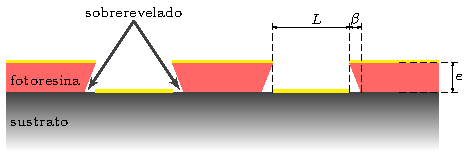
\includegraphics[width=\textwidth]{Esquemas/altura-ancho.pdf}
 				\end{subfigure}
 				\begin{subfigure}[t]{0.86\textwidth}
 				\includegraphics[width=\textwidth]{Imagenes/fotoresina_perfil.jpg}
 				\end{subfigure}
 				\caption[Perfil de fotorresina para el decapado o\textit{ lift-off}]{Arriba: esquema de la fotoresina depositada y revelada, donde se muestra la relación de espesor respecto del ancho de línea y el sobrerevelado necesario para un correcto decapado. Abajo: corte por FIB para evaluar el sobrerevelado y espesor obtenido luego de la transferencia por litografía.}
 				\label{fig:undercut}
 				\end{figure}

 	   		 La variable más delicada es, sin lugar a dudas, el tiempo de revelado, ya que es la que compensa los errores acumulados en el proceso. Cualquier irregularidad en el sistema de iluminación, inhomogeneidades en el espesor o calentamiento desparejo se ve reflejado en tiempos de revelado diferenciales para diferentes sectores. Dicho esto, mientras más extenso el sustrato, más difícil es lograr un revelado homogéneo. Es también en este paso donde se regula el <<sobrerevelado>> o, del inglés \textit{undercutting}, perfil necesario para que no se deposite metal en los laterales de la fotorresina (figura \ref{fig:undercut}). El parámetro $\beta$ es la medida del sobrerevelado, que es la diferencia entre la proyección en el sustrato de la superficie superior y la superficie inferior de la resina. Un $\beta\!\!\approx$\SI{500}{\nm} es el ideal para obtener buenos resultados en el procesos de \textit{lift-off}. 
 
 	         En la secuencia de imágenes de microscopia óptica de la figura \ref{fig:revelado} se muestra cómo evoluciona el revelado con el tiempo y, en particular, se ve en la última imagen de esta secuencia, el resultado final de la etapa de litografía y cómo el diseño resultó transferido de manera precisa.

 				%Imagnes revelado
 				\begin{figure}[h!]
			 	   	    \centering
			 	   	    \begin{subfigure}[t]{0.495\textwidth}
			        	\includegraphics[width=\textwidth]{Imagenes/revelado1.jpg}
			       		\end{subfigure}
			     		\begin{subfigure}[t]{0.495\textwidth}
			     		\includegraphics[width=\textwidth]{Imagenes/revelado2.jpg}
			    		\end{subfigure}
			     		\begin{subfigure}[t]{0.495\textwidth}
						\vspace*{-0.3cm}
			     		\includegraphics[width=\textwidth]{Imagenes/revelado3.jpg}
			        	\end{subfigure}
						\begin{subfigure}[t]{0.495\textwidth}
			     		\vspace*{-0.3cm}
			     		\includegraphics[width=\textwidth]{Imagenes/revelado4.jpg}
			        	\end{subfigure}
			     		\caption[Revelado en función del tiempo]{Tiempos crecientes de revelado: \SI{2.5}{min}, \SI{3.5}{min}, \SI{4.5}{min} y \SI{6}{min}). Se aprecia como se disuelve la resina en la solución reveladora indicado por el cambio de color a medida que disminuye el espesor. Se muestra en la última microscopía el revelado completo con un 20\% de tiempo adicional para crear el perfil negativo de las paredes, necesario para el proceso de\textit{ lift-off}.}
			     		\label{fig:revelado}
			     	   	\end{figure}

			  \vspace*{2mm}Se llevó a cabo una segunda etapa de litografía (luego del depósito de Ti\textbar Au para los electrodos) para colocar una resina fotocurable, epoxi, de alta viscosidad que genera estructuras de hasta \SI{100}{\um} de altura. En la fotografía de la figura \ref{fig:su8} se destaca la alta viscosidad de la misma al momento de hacer el depósito por \textit{spincoating}. Nuevamente, los datos del proceso se obtuvieron de la hoja de datos del fabricante\cite{Su8,Microchemicals2014} y los detalles experimentales fueron expuestos en  la sección \ref{sec:fotolito}, pág. \pageref{sec:fotolito}. \pagebreak   Esta resina se usó para hacer la celda electroquímica, la cual puede contener un volumen aproximado \SI{2}{\ul} de solución. En las microscopías ópticas de la figura \ref{fig:resultados-su8} se muestra el resultado obtenido luego de alinear y depositar esta resina epoxi.

			  	\begin{figure}[th!]
 				\centering
 				\includegraphics[width=\textwidth]{Imagenes/SU8.jpg}
 				\caption[Depósito de la resina epoxi SU8]{Depósito por \textit{spin-coating }de la resina expoxi para encapsular los multisensores. Se destaca la alta viscosidad de la misma, lo que permite formar paredes de hasta \SI{100}{\um} de espesor.}
 				\label{fig:su8}
 				\vspace*{6mm}
 				\end{figure}
 		
 				\begin{figure}[th!]
			 	   	    \centering
			 	   	    \begin{subfigure}[t]{0.495\textwidth}
			        	\includegraphics[width=\textwidth]{Imagenes/alineacionSU8.pdf}
			       		\caption{Alineación de la segunda máscara con la película de Ti\textbar Au ya depositada.}
			         	\label{fig:alineacion}
			     		\end{subfigure}
			     		\begin{subfigure}[t]{0.495\textwidth}
			     		\includegraphics[width=\textwidth]{Imagenes/DIE-SU8.pdf}
			    		\caption{Microscopía de uno de los multisensores con la celda integrada.}
			     		\label{fig:die-su8}	
						\end{subfigure}
						\caption[Alineación y celda integrada en SU8]{Resultados de la alineación de la capa de los electrodos con la máscara para transferir la fotoresina epoxi (a) y, (b) detalle de un sensor terminado con celda EQ.}
			     		\label{fig:resultados-su8}
			     	   	\end{figure}

	\subsection{Películas delgadas de Au}

		 Como ya se mencionó anteriormente, los electrodos de los sensores son de Au y fueron depositados por la técnica de pulverización catódica, más comúnmente conocida por su nombre en inglés \textit{sputtering}. La fabricación consistió primero en depositar una capa de al menos de \SI{20}{\nm} de espesor, llamada capa de  adherencia, que puede ser indistintamente de Ti o Cr, la cual promueve la adherencia del Au; sin esta capa el Au no adhiere sobre superficies no metálicas.\cite{Hieber1976} Una vez depositada la capa adherente y sin romper el vacío de la cámara del equipo, se depositaron \SI{150}{nm} de Au. El espesor resultó ser el óptimo para lograr un electrodo mecánicamente robusto y con buenas propiedades de conducción eléctrica pero suficientemente delgado para que las películas delgadas mesoporosas sean continuas entre los electrodos y el sustrato. Para cada caso, en condiciones constantes, se puede realizar una curva de calibración. La misma se consigue graficando el espesor de las películas depositadas en función del tiempo de depósito, con el objetivo de establecer la velocidad de depósito y así poder controlar el espesor de la película. 

		 Se optimizaron las condiciones de \textit{sputtering} para obtener películas homogéneas tanto en espesor como superficialmente. Para lograrlo se variaron los parámetros relevantes de la técnica: aceleración de los iones, determinada por diferencia de tensión entre el cátodo y ánodo, densidad de corriente y el flujo de Ar. Una vez establecidas dichas condiciones se mantuvieron constante a lo largo del trabajo de tesis. El espesor de las películas metálicas, $d$, se reguló controlando el tiempo de depósito, $t$. De acuerdo a los los trabajos de Sigmund\cite{sigmund1968} y Seah\cite{Seah2005} estas variables son directamente proporcionales entre sí y están vinculadas por la ecuación \ref{eq:sputt}, donde $J$ es la densidad de corriente, $Y$ el rendimiento de la pulverización, $r$ el radio atómico del material y $e_o$ la carga del electrón.

	 			\begin{equation}
	 				d=\left(\frac{JYr^3}{e_o}\right)t
	 				\label{eq:sputt}
	 			\end{equation}

		 Las condiciones de depósito de cada una de las sucesivas capas se detallan en la tabla \ref{tabla:sputt1}, pág. \pageref{tabla:sputt1}, para las películas metálicas y en la tabla  \ref{tabla:sputt2}, pág. \pageref{tabla:sputt2}, para el SiO$_2$. 

		 Para establecer la velocidad de depósito de cada uno de los materiales pulverizados, se midió el espesor resultante de las películas por diferentes técnicas. Para monocapas de Au y espesores pequeños típicamente menores a los \SI{30}{\nm}, se utilizó elipsometría espectrométrica; los detalles experimentales y la base de la técnica ya fueron discutidos en la sección \ref{sec:elipso}, pág. \pageref{sec:elipso}. Para evaluar el apilamiento de sucesivas capas, inspeccionar la homogeneidad transversal y superficial y medir el espesor de cada una de las capas, se tomaron imágenes de MEB asistida por microscopía FIB. Esta técnica permite hacer cortes en el sentido normal al plano de las películas en cualquier área seleccionada.
		
		 En la figura \ref{fig:FIB_electrodos} se puede ver un corte transversal de los electrodos, realizado por FIB, donde se ven los espesores de ambas películas metálicas (Ti y Au), así como la capa dieléctrica de SiO$_2$. También se aprecia la buena homogeneidad en el espesor de cada una de las capas y en la superficie de la capa de Au, donde ocurrirá finalmente el intercambio electrónico entre las especies rédox. Midiendo los espesores de las capas depositadas a distintos tiempos, podemos establecer la velocidad de depósito, obtenida de la pendiente de la figura \ref{fig:calibracionAu}. Como ya se mencionó en reiteradas ocasiones, es de suma importancia conocer y controlar los espesores de cada una de las capas, ya sean películas delgadas mesoporosas, densas o metálicas.


		 		%figura FIB de los electrodos
						  \begin{figure}[th!]
						  \begin{center}
						  \includegraphics[width=0.80\textwidth]{Imagenes/Perfil.jpg}
						  \caption[Sección trasversal de los eletrodos]{Corte transversal de los electrodos, donde se observan detalles de la bicapa Cr\textbar Au depositada sobre una oblea de silicio con un depósito aislante de SiO$_2$.}
						  \label{fig:FIB_electrodos}
						  \end{center}
						  \end{figure} 	

				%Grafico de la curva de calibración para el Au
					   		\begin{figure}[th!]
					   		\begin{center}
							\includegraphics[width=0.75\textwidth]{Graficos/Espesor_Au.pdf}
							\caption[Curva de calibración para el espesor de los electrodos]{Curva de calibración para establecer la velocidad de depósito de la capa de Au. La misma se realizó por pulverización catódica en las condiciones experimentales detalladas en la tabla \ref{tabla:sputt1}.}
							\label{fig:calibracionAu}
							\end{center}
							\end{figure}		  
		
	\subsection{Decapado de la fotorresina o\textit{ lift-off}}

		 La última etapa de la fabricación de los electrodos es el decapado de la fotorresina, técnica que se conoce más comúnmente con el nombre en inglés, \textit{lift-off}. Consiste en disolver la fotorresina que queda luego del revelado y que se utilizó a modo de capa de sacrificio. En la figura \ref{fig:undercut} se pueden ver los sitios por donde da comienzo la disolución. La fotoresina utilizada es completamente soluble en acetona. Cabe destacar, nuevamente, que es importante la discontinuidad de la película de oro para que tenga éxito esta etapa, ya que, si existe continuidad entre la parte que se quiere dejar y la que no, se generan imperfecciones en los bordes, o se desprende el metal de partes que no se desea. Para ello es muy importante saber bien los espesores que se logran durante el depósito, tanto de fotorresina como de película de Au, para regular la distancia que quede entre el metal en el sustrato y el metal sobre la resina. El esquema y la microscopía de la figura \ref{fig:undercut} presentado anteriormente en la pág. \pageref{fig:undercut} ejemplifica bien esta situación.

					  %Oblea Terminada V1
					  \begin{figure}[ht!]
					  \begin{center}
					  \includegraphics[width=\textwidth]{Imagenes/lift-off.jpg}
					  \caption[Proceso de decapado o\textit{ lift-off}]{Proceso de decapado o\textit{ lift-off}. Fotografía correpondiente a los electrodos del primer diseño, donde se muestra como a medida que se disuelve la fotorresina se va levantando el metal que está sobre ella.}
					  \label{fig:ultrasonido}
					  \end{center}
					  \end{figure}

		 Por último, es importarte recalcar que es necesario aplicar ultrasonido para un procesado eficiente. No alcanza con una simple inmersión de la oblea en solvente sino que se precisa mantener una constante convección en baño ultrasónico para la completa remoción de la fotorresina. A su vez, este proceso de constante movimiento evita el redepósito del metal liberado sobre los electrodos (figura \ref{fig:ultrasonido}), ya que si ocurre este fenómeno es muy difícil, una vez que se seca la oblea, remover el metal de desperdicio que se adhiere a los electrodos. Es en esta etapa final del proceso donde se demuestra si resultaron efectivas las etapas de limpieza y revelado. De haber algún residuo remanente durante la limpieza del sustrato o haber efectuado un revelado incompleto, se producirá indefectiblemente el desprendimiento de los electrodos del sustrato.

		 Finalmente, en las figuras \ref{fig:ObleaV1} y \ref{fig:ObleaV2}, se muestra el resultado final de la fabricación de los electrodos realizados en obleas de cuatro pulgadas (\SI{10}{\cm} de diámetro) para los dos diseños elaborados.\pagebreak
		

		 			  \clearpage
					  %Oblea Terminada V1
					  \begin{figure}[ht!]
					  \begin{center}
					  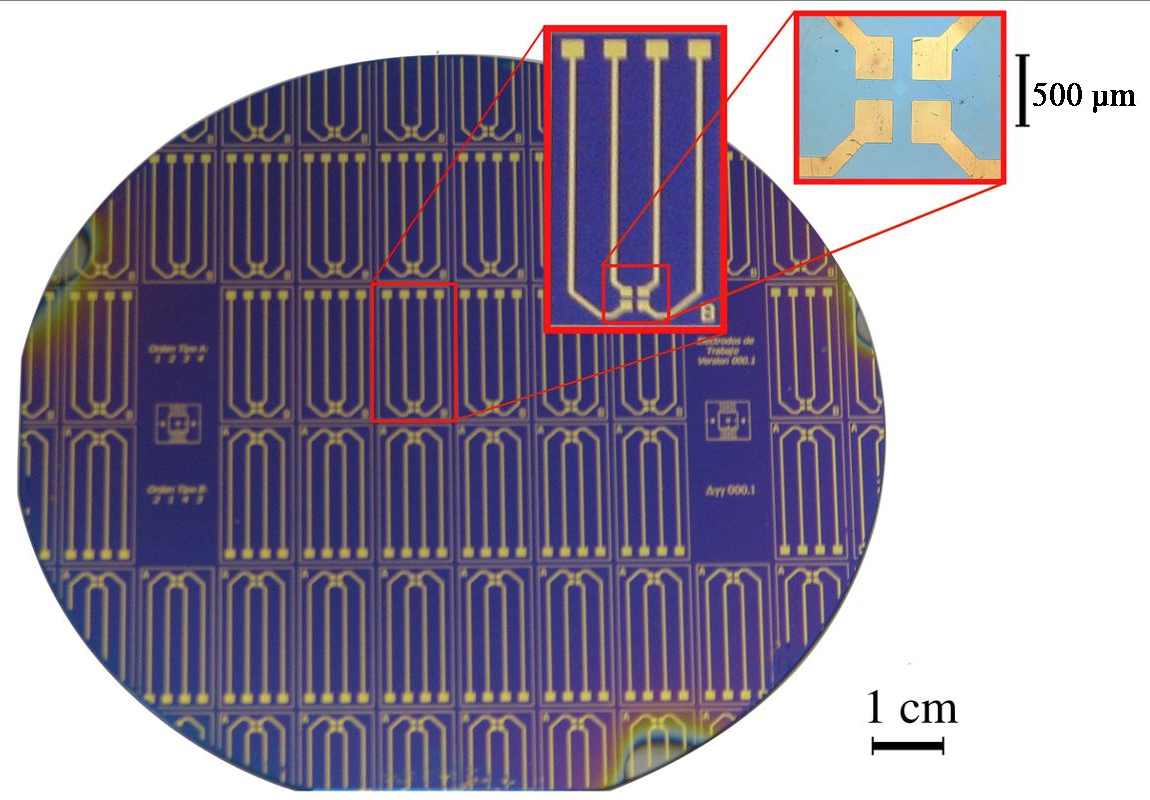
\includegraphics[width=\textwidth]{Imagenes/ObleaV1.jpg}
					  \caption[Electrodos, primera versión]{Primer diseño de los sensores. Oblea de silicio de \SI{10}{cm} de diámetro, capa de SiO$_2$ y 32 sensores con cuatro electrodos de trabajo cada uno.}
					  \label{fig:ObleaV1}
					  \end{center}
					  \end{figure} 	

					  %Oblea Terminada V2
					  \begin{figure}[h!]
					  \begin{center}
					  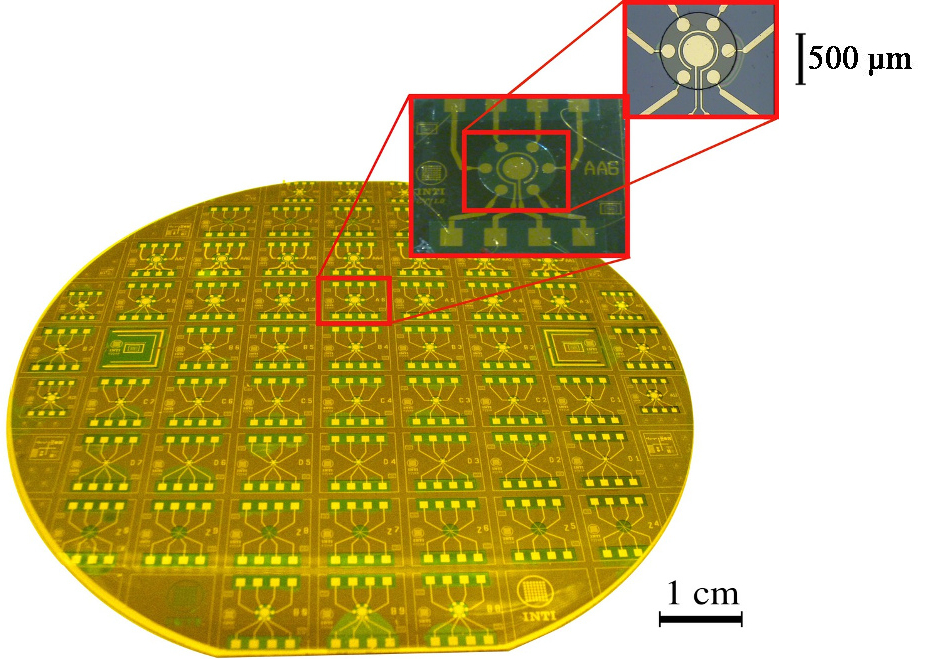
\includegraphics[width=\textwidth]{Imagenes/ObleaV2.jpg}
					  \caption[Electrodos, segunda versión]{Segundo diseño de los sensores. Oblea de silicio de \SI{10}{cm} de diámetro con 46 sensores con 6 electrodos de trabajo, contraelectrodo y pseudoreferencia. También se muestra la celda electroquímica depositada con resina epoxi SU-8.}
					  \label{fig:ObleaV2}
					  \end{center}
					  \end{figure} 	
	
\section{Incompatibilidad \textit{top-down/bottom-up}}

  			Lo primera acción que se llevo a cabo luego de fabricar los electrodos fue la de evaluar su desempeño electroquímico. Para ello se utilizaron sondas rédox de uso regular en electroquímica. En la sección \ref{sec:respuesta_sondas_au} se demostró que el desempeño de los electrodos es analíticamente satisfactorio para su uso en sensores. La siguiente etapa del trabajo de tesis consintió en el depósito de la película mesoporosa sobre los electrodos. Esta etapa se expuso y se discutió a lo largo del capítulo \ref{chap:Mesoporosos}, abordando las técnicas de depósito, el control sobre la síntesis, los parámetros para obtener películas de diferente porosidad, espesor, adherencia, etc.

  			Previo a los resultados discutidos y analizados en el capítulo \ref{chap:Mesoporosos} y basándose en trabajos similares\cite{Otal2006,Calvo2009,Fattakhova-Rohlfing2007,Rohlfing2005}, donde utilizan mediciones electroquímicas como herramienta para establecer propiedades de las \pdm, se realizaron experimentos preliminares y equivalentes para evaluar el transporte en películas delgadas mesoporosas de SiO$_2$. En los trabajos citados utilizan vidrio ITO o vidrio FTO como electrodos y llevan a cabo mediciones electroquímicas sobre sistemas clásicos, películas calcinadas y electrodos no miniaturizados. En este trabajo las primeras medidas se realizaron sobre películas mesoporosas de SiO$_2$ estructuradas con F127, depositadas sobre películas delgadas de Au, y tratadas por la vía de calcinación (\SI{350}{\celsius}). Los resultados preliminares de estas mediciones (previos al desarrollo de la discusión sobre transporte del capítulo \ref{chap:Electroquimica}) no fueron los esperados. Mostraban, o bien voltagramas <<planos>>, o bien curvas donde la respuesta no era óptima, propia de electrodos con alta resistencia o limitados en la cinética de transferencia electrónica, tal como se muestra en los voltagramas de la figura \ref{fig:volta_chotos}.

  				\begin{figure}[ht]
		 	      \begin{subfigure}[t]{0.495\textwidth}
		          	\includegraphics[width=\textwidth]{Graficos/Fe-Au-chotos.pdf}
		      		\end{subfigure}
		      	 \begin{subfigure}[t]{0.495\textwidth}
		          	\includegraphics[width=\textwidth]{Graficos/Ru-Au-chotos.pdf}
		 			\end{subfigure}
		      	 \caption{Voltametrías para \ferroferri\space (izquierda) y \aminorutenio\space (derecha) tomados a \SI{50}{\milli\volt\per\second} sobre electrodos de Au calcinados, en los cuales la respuesta es deficiente para ambas sondas, producto de una transferencia electrónica impedida.}
		      	 \label{fig:volta_chotos}
	      		 \end{figure}	

  			 \vspace*{2mm}El estudio de porqué la respuesta era muy diferente a la reportada para estos sistemas calcinados se abordó de forma sistemática. Se plantearon cuatro hipótesis: 1) contaminación de los reactivos, 2) poros bloqueados, 3) difusión de impurezas y, 4) reestructuración de la superficie de los electrodos de Au. Las dos últimas como consecuencia directa del proceso de calcinación.

  			 Para evaluar la hipótesis de contaminación en los reactivos, se repitió la preparación de los soles, de las soluciones con las sondas, se reemplazaron los solventes y el electrolito soporte por nuevos reactivos. La respuesta electroquímica seguía siendo deficiente por lo que se descartó esta hipótesis. 

  			 Las hipótesis de poros bloqueados quedó descartada luego de realizar repetidas mediciones de eliposoporosimetría ambiental demostrando la buena accesibilidad y porosidad que mostraban las películas delgadas mesoporosa sometidas a  calcinación (ver sección \ref{sub:m_todo_de_calcinaci_n}, pág. \pageref{sub:m_todo_de_calcinaci_n} y figura \ref{fig:F127_epa_psd_cal}, pág. \pageref{fig:F127_epa_psd_cal}).

  			 Para evaluar las hipótesis de contaminantes que difunden hacia la superficie y reestructuración del Au, ambos fenómenos debido a la temperatura de calcinacinación, se llevaron a cabo experimentos con muestras control, las cuales consistieron en electrodos de Au sometidos a calcinación pero sin depositar películas mesoporosas sobre ellos. En resumen, se sometió los electrodos de Au desnudos a condiciones de humedad y temperatura idénticos a las utilizadas en el proceso de síntesis de las \pdm\space (ver el proceso descrito en la sección \ref{sec:cond_y_extr}, pág. \pageref{sec:cond_y_extr}). La respuesta electroquímica seguía siendo defectuosa, por lo que se consolidaron las hipótesis de difusión de contaminantes o reestructuración (producto de la temperatura a la que fueron sometidos los electrodos) como causante de dicha respuesta. Las próximas secciones abordan la temática sobre cada una de las hipótesis.

	\subsection{Reestructuración de la superficie de los electrodos}
			  		
			 Se estudió la morfología de las películas delgadas de Au en busca de cambios estructurales producto de someter los electrodos a calcinación. Se tomaron imágenes por MEB las cuales se exponen en la figura \ref{fig:Au_compTT}. Allí se comparan depósitos de Cr\textbar Au tratados térmicamente con depósitos de de Cr\textbar Au no tratados. Se observa un crecimiento en el tamaño de partícula para los sometidos a tratamiento térmico, más específicamente a \SI{350}{\celsius}, temperatura usada para la vía clásica de síntesis de \pdm. Este hecho demuestra que esta temperatura es suficiente para, al menos, producir un aumento en el tamaño de los cristales de las películas delgadas de oro. Dicha transformación también fue reportada a una temperatura menor (\SI{300}{\celsius})	 por \v{S}vor\v{c}\'ik y colaboradores.}\cite{Svorcik2010}. 

			 		\begin{figure}[th]
		 	   	    \begin{subfigure}[t]{0.495\textwidth}
			       	\includegraphics[width=\textwidth]{Imagenes/Au-sinTT.jpg}
			   		\end{subfigure}
			   		\begin{subfigure}[t]{0.495\textwidth}
			   	    \includegraphics[width=\textwidth]{Imagenes/Au-conTT.jpg}
			   		\end{subfigure}
					 \caption[Microscopía comparativa electrodos Au]{Microscopías de barrido electrónico donde se comparan los electrodos sin calcinar (izquierda) con aquellos sometidos a tratamiento térmico (derecha) . Se observa en las películas calcinadas un aumento en el tamaño de las partículas de Au.}
					 \label{fig:Au_compTT}	
				     \end{figure}	

		     \vspace{2mm}Con el propósito de determinar si esta reestructuración, debida al tratamiento térmico,  afecta las propiedades eléctricas de las películas delgadas de Au se midió la resistencia superficial de las mismas. Un aumento en la resistividad puede traer aparejadas deformaciones en los voltagramas, caída óhmica o separación de los potenciales de pico. Las mediciones se llevaron a cabo sobre tres muestras: una sin tratamiento térmico, otra calcinada a \SI{350}{\celsius} y una tercera llevada también a \SI{350}{\celsius} pero en atmósfera de alto vacío (\SI{e-5}{\milli\bar}). Los resultados se resumen en la tabla \ref{tabla:resistencia}, donde se corrobora que la resistencia por cuadrado aumenta para las muestras sometidas a tratamiento térmico, posiblemente debido a la reestructuración o a la difusión de impurezas hacia la superficie. Dichas impurezas pueden provenir del Au, de la capa de adherencia o del sustrato (silicio o vidrio).

				\begin{table}[ht!]
			  		  \caption[Resistencia superficial de los electrodos]{Resistencia superficial de los electrodos con y sin tratamiento térmico.} 
			  		  \begin{tabular}{>{\raggedright\arraybackslash}m{4.2cm}>{\raggedright\arraybackslash}m{7.075cm}} 
			  		  \toprule
					  Muestra & Resistividad superficial $(\Omega/_{\square})$  \\ \midrule
			      	  Au \SI{350}{\celsius} 		  	& $3.720 \pm 0.001$		 \\	  
			      	  Au \SI{350}{\celsius} en vacío	& $3.685 \pm 0.001$		 \\	  
			      	  Au \SI{25}{\celsius}    	  		& $0.595 \pm 0.001$		 \\ 
			      	  \bottomrule
			    	  \end{tabular}
			    	  \label{tabla:resistencia}
			   		  \end{table}	
	
	\subsection{Difusión de contaminantes}

			Se ha reportado trabajos donde se demuestra que es posible la difusión hasta la superficie del electrodo, de metales provenientes de la capa de adherencia e incluso de iones provenientes del sustrato \cite{Alonso1990,Moody2003}. Para ello se decidió analizar la superficie de los electrodos mediante espectroscopía de fotoelectrones emitidos por rayos X (XPS). Se llevó a cabo un experimento en el cuál se depositaron dos electrodos de Cr\textbar Au sobre silicio, uno de ellos fue sometido a tratamiento térmico mientras que el otro no. Los resultados se presentan en el gráfico de la figura \ref{fig:XPS}, donde observa la presencia de picos de cromo ligado a oxígeno, demostrando la difusión hacia la superficie de cromo.
				
				\begin{figure}[hb!]
		 	       	\begin{center}
		 	       	\includegraphics[width=0.95\textwidth]{Graficos/XPS.pdf}
		        	\caption[XPS de películas delgadas de Cr\textbar Au]{Espectroscopía de fotoelectrones emitidos por rayos (XPS) correspondiente a películas delgadas de Cr\textbar Au con y sin tratamiento térmico. Obsérvese los picos correspondiente al cromo y el aumento de la intensidad relativa del pico correspondiente al oxígeno, sugiriendo la difusión de Cr$_x$O$_y$ hacia la superficie de los electrodos.}
		         	\label{fig:XPS}
		         	\end{center}
		     		\end{figure}

			%
			Esto sugiere que el cromo, utilizado como capa de adherencia, se oxida y puede difundir hacia la superficie del electrodo cuando éstos son sometidos a una temperatura de \SI{350}{\celsius}.

			Una vez demostrado que es posible la difusión de impurezas a \SI{350}{\celsius}, que provengan tanto del Au como de la capa de adherencia, se fabricó una tanda de electrodos utilizando oro de mayor pureza, Au4N (99,99\% de \textit{Sigma Aldrich}) en lugar del Au3N (99,9\% de \textit{Eurometal}), el cual es mucho más económico, fácil de conseguir y es el blanco habitual para pulverización disponible en el laboratorio de películas delgadas del INTI. El propósito de estas caracterizaciones es el de discriminar si las impurezas provienen del Au o del Cr y ver como es afectada la respuesta electroquímica, ya que la voltametría cíclica (VC) es una técnica analítica cuya respuesta depende fuertemente de la superficie del electrodo.\cite{Wi2000,Pumera2007,Gewirth2004,Villullas2000}

			En los voltagramas de la figura \ref{Fig:Comparacion-Au} se expone la respuesta electroquímica  para \ru\space y \fe\space utilizando electrodos Au3N calcinados y sin calcinar con aquella obtenida para electrodos de Au de mayor pureza (Au4N), estos últimos tratados a \SI{350}{\celsius}. 

				\begin{figure}[ht]
		 	      \begin{subfigure}[t]{0.495\textwidth}
		          	\includegraphics[width=\textwidth]{Graficos/Fe-Au-Comparaciones.pdf}
		         	\caption{Voltametrías cíclicas para \fe\space \SI{1}{\milli\Molar} tomadas a \SI{50}{\milli\volt\per\second} en una solución \SI{0.1}{\Molar} de KCl.}
		          	\label{fig:Fe-Au-compa}
		      		\end{subfigure}
		      	 \begin{subfigure}[t]{0.495\textwidth}
		          	\includegraphics[width=\textwidth]{Graficos/Ru-Au-Comparaciones.pdf}
		         	\caption{Voltametrías cíclicas para \ru\space \SI{1}{\milli\Molar} tomadas a \SI{50}{\milli\volt\per\second} en una solución \SI{0.1}{\Molar} de KCl.}
		          	\label{fig:Ru-Au-compa}
		      		\end{subfigure}
		      	 \caption[Comparación entre electrodos calcinados y sin calcinar]{Voltametrías para \ferroferri\space y \aminorutenio\space donde se compara la respuesta sobre electrodos de Au4N calcinado (\usebox{\negro}) con electrodos de Au3N calcinado (\usebox{\punteado}) y Au3N sin calcinar (\usebox{\rojo}). Se observa una respuesta deficiente solo para electrodos de Au3N sometidos a calcinación.}
		      	 \label{Fig:Comparacion-Au}
	      		 \end{figure}	

			La primera observación que se desprende de los voltagramas es que la respuesta para el Au3N sin tratamiento térmico es prácticamente idéntica a la del Au4N con tratamiento térmico. Por otro lado la respuesta del oro menos purificado, Au3N, sometida a temperatura, muestra una clara irreversibilidad en los procesos de oxido reducción para ambas sondas, a tal punto que no se observa la reducción para \ferroferri\space (figura \ref{fig:Fe-Au-compa}, curva punteada).  

		    Con estos resultados y lo expuesto anteriormente, se demostró que durante la calcinación de Au3N se produce una reestructuración de la superficie de los electrodos, aumenta la resistencia eléctrica y pueden difundir impurezas o átomos de la capa de adherencia hacia la superficie. 

		    De la comparación entre electrodos fabricados con Au3N y Au4N, ambos con Cr de igual calidad como capa de adherencia, se puede concluir que la respuesta electroquímica anómala es debida a una capa superficial de impurezas, generada por un proceso difusivo durante el tratamiento térmico. Dicha difusión dificulta la transferencia electrónica entre sonda\textbar electrodo, alejándose de la idealidad y generando una amplia separación de potenciales entre los picos anódico y catódico. A pesar de que se atribuye a que la transferencia electrónica se encuentra impedida por las impurezas en el propio Au, también se demostró que es posible la difusión del Cr, hecho que obliga a considerar la calidad de la capa de adherencia que se utiliza ya sea de cromo u otro metal. Como consecuencia directa de estos procesos difusivos se obtiene una respuesta EQ deficiente y no reproducible. Este resultado fue uno de los que motivó el desarrollo de películas delgadas mesoporosas a bajas temperaturas cuyos resultados fueron expuestos en el capítulo \ref{chap:Mesoporosos}.

\section{Multisensores de respuesta selectiva}

			Una vez hallado el motivo de la respuesta electroquímica no deseada, surgieron, naturalmente, dos vías de acción: 1) cambiar el material de los electrodos por Pt u Au de mayor calidad, y 2) sustituir o evitar la etapa de calcinación en la condensación y extracción de películas delgadas mesoporosas.

				\begin{figure}[b!]
		 	       	\begin{center}
		 	       	\includegraphics[trim=0 0 0 0.3cm, width=\textwidth]{Esquemas/sensorito-esquema.pdf}
		        	\caption[Esquema de sensores EQ selectivos]{Microscopía óptica de un sensor con múltiples electrodos recubiertos con películas delagadas mesoporosas de Si$_{0.9}$Zr$_{0.1}$O$_2$. Uno se dejó sin recubrir mientras que dos fueron funcionalizados con DHDP y APTES respectivamente. A modo ilustrativo se muestra un esquema de la estructura de las películas en cada caso y una típica respuesta EQ para cada uno de ellos.}
		         	\label{fig:sensor-calesita}
		         	\end{center}
		     		\end{figure}

			Ambas alternativas fueron puestas en prácticas con resultados exitosos. Se consideró la segunda opción mucho más rica, tanto científica como tecnológicamente, ya que permite minimizar los procesos difusivos, disminuir costos y, a su vez, desarrollar un método de condensación y extracción para sintetizar películas delgadas mesoporosas de óxido de silicio a temperaturas menores a \SI{130}{\celsius}. 

			En este tópico, la literatura especializada es escasa, y dicho desarrollo condujo al estudio de las matrices porosas resultantes, de la condensación de la fase inorgánica y de la extracción de la fase orgánica, así como también al estudio sobre la termodinámica y la cinética de transporte con sondas electroquímicas, temas tratados extensamente en los capítulos  \ref{chap:Mesoporosos} y \ref{chap:Electroquimica}. 

    		En esta sección se capitalizan las herramientas y conocimientos adquiridos sobre estos temas aplicados al uso de los multisensores, conceptualizando el uso de electrodos con diferentes respuestas que funcionan cooperativamente en la detección de las sondas modelos que se utilizaron a lo largo del trabajo de tesis. 

			Sobre un multisensor fabricado a partir del diseño <<calesita>>, se depositaron películas delgadas mesoporosas de Si$_{0.9}$Zr$_{0.1}$O$_2$ por el método de alto vacío (Vac\pdmZ). Uno de los seis electrodos de trabajo se enjuagó con un hisopo con etanol para remover la película de óxido. Luego se llevaron a cabo, individualmente sobre dos electrodos, las funcionalizaciones con DHDP y APTES descritas en la sección \ref{sub:funcionalizaci_n_de_las_pdm}, pág. \pageref{sub:funcionalizaci_n_de_las_pdm}. Sobre ese mismo sensor se tomaron las mediciones electroquímicas, de las cuales se pueden obtener cuatro respuestas por sensor: del electrodo de Au sin recubrir, del recubierto con Vac\pdmZ\space y de los dos recubiertos con Vac\pdmZ\space funcionalizados con APTES y DHDP (Vac\pdmZ$^N_1$\space y  Vac\pdmZ$^P_3$). El diagrama de la figura \ref{fig:sensor-calesita} representa en forma esquemática esta situación mostrando el tipo de recubrimiento de cada electrodo y respuestas típicas que podrían obtenerse al colocar un analito electroactivo. 

			En las próximas secciones se analizará la respuesta del multisensor para cada una de las sondas ensayadas y se discutirán algunas formas de análisis multivariable para el tratamiento de los datos. 

	\subsection{Respuesta para \ru, \fe\space y \fc\space sobre multisensores}	

		Durante el desarrollo del capítulo \ref{chap:Electroquimica} se estudió e interpretaron los voltagramas para cada una de estas sondas, cabe destacar que en dicho capítulo la mayoría de los datos fueron tomados sobre electrodos sin litografiar, mientras que en esta sección los datos fueron medidos sobre un único multisensor. Ya sea que estén o no litografiados los voltagramas son equivalente para ambas plataformas. En esta sección se explota la información que se pueda extraer de cada voltagrama, resumiendo los datos en graficos de distintos tipos.

		Se analizó la respuesta electroquímica de \aminorutenio, \ferroferri\space y \ferroceno\space para cada uno de los electrodos de un multisensor EQ similar al mostrado en el esquema de la figura \ref{fig:sensor-calesita}. La medición consiste en ciclar electroquímicamente, en un rango de potencial adecuado para cada sonda, utilizando cada uno de los electrodos de un mismo multisensor. Una vez que se colectaron los $n$ voltagramas se extrae de cada uno de ellos el pico de máxima densidad de corriente anódica, luego se gráfica dicho valor en función de la cantidad de ciclos normalizado por la densidad de corriente del electrodo de Au desnudo ($\text{j}_p/\text{j}_p^\text{Au}$).
		
		En el caso del \fe\space se tiene una fuerte exclusión por parte de las películas sin funcionalizar y una mínima permeación en las películas con APTES y DHDP. 
		En el caso del \fc\space en todos las casos el fenómeno dominante es la permeación, como es de esperar para una sonda de carga neutra. Debido a que las membranas fueron condensadas y extraídas a bajas temperaturas la difusión es lenta y la corriente resultante es bastante menor que la obtenida en electrodos de Au desnudo (consultar sección \ref{sec:difusion}, pág. \pageref{sec:difusion}). Las corriente de pico a lo largo de los ciclos para estas dos sondas es prácticamente invariante tal como se puede observar en los gráficos de la figura \ref{fig:ciclos-fe-fcoh}.

			\begin{figure}[h!]
		 	\begin{subfigure}[t]{0.495\textwidth}
		 	  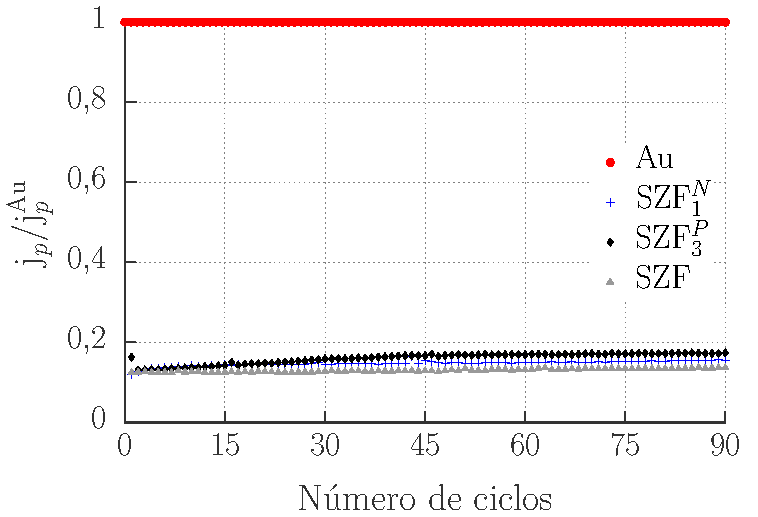
\includegraphics[trim=0 0 0 0.5cm,width=\textwidth]{Graficos/ciclosintferroceno.pdf}
		      \end{subfigure}
			\begin{subfigure}[t]{0.495\textwidth}
		 	    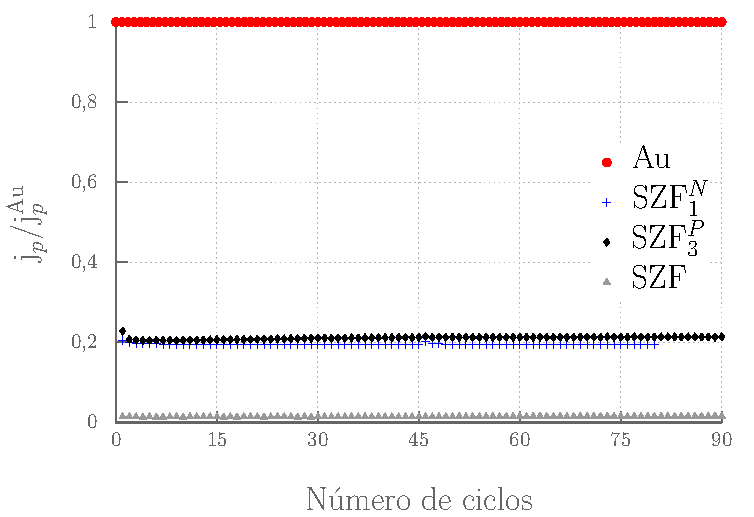
\includegraphics[trim=0 0 0 0.5cm,width=\textwidth]{Graficos/ciclosintfecn.pdf}
			\end{subfigure}
		      	\caption[Corriente de pico de \fc\space y \fe\space en función del número de ciclos]{Corriente de pico anódico normalizada para \fc\space \SI{1}{\milli\Molar} (izquierda) y  \fe\space \SI{1}{\milli\Molar} (derecha) en función de la cantidad de ciclos. Los datos fueron tomados a una velocidad de barrido de \SI{50}{\milli\volt\per\second} en solución de KCl \SI{100}{\milli\Molar} en un multisensor compuesto por cuatro electrodos diferentes: de Au (Au), recubierto con una película mesoporosa sin funcionalizar (\pdmZ), con una funcionalizada con DHDP (\pdmZ$^P_3$) y con una funcionalizada con APTES (\pdmZ$^N_1$).}
		      	\label{fig:ciclos-fe-fcoh}
		      	\end{figure}

		     \begin{figure}[b!]
		 	       	\begin{center}
		 	       	\includegraphics[trim=0 0 0 1cm, width=0.85\textwidth]{Graficos/ciclosintru.pdf}
		        	\caption[Corriente de pico de \ru\space en función del número de ciclos]{Corriente de pico anódico para \ru\space \SI{1}{\milli\Molar} en función de la cantidad de ciclos. Los datos fueron tomados a una velocidad de barrido de \SI{50}{\milli\volt\per\second} en solución de KCl \SI{100}{\milli\Molar} en un sensor compuesto por cuatro electrodos diferentes: de Au (Au), recubierto con una película mesoporosa sin funcionalizar (\pdmZ), con una funcionalizada con DHDP (\pdmZ$^P_3$) y con una funcionalizada con APTES (\pdmZ$^N_1$).}
		         	\label{fig:ruciclos}
		         	\end{center}
		     		\end{figure}

	    El caso más interesante es de la sonda positiva, el \ru. La intensidad de pico anódico, para condiciones de contorno constante (velocidad de barrido, pH, fuerza iónica, concentración de \ru\space en solución), evoluciona en cada ciclo de forma diferente según se va adsorbiendo en las películas delgadas mesoporosas. La interpretación de las distintas respuestas ya se discutieron en la sección \ref{sub_sec_funcionalizaciones_chap_4}, pág. \pageref{sub_sec_funcionalizaciones_chap_4}. Al\space igual que para las otras sondas, en el gráfico \ref{fig:ruciclos}  se muestra cómo va cambiando la intensidad de pico, para cada electrodo, a medida que se aumenta la cantidad de ciclos electroquímicos. 

	\subsection{Análisis multivariable de la respuesta electroquímica}	     		

	 Con el objetivo de utilizar los sensores en aplicaciones analíticas se sintetizaron aún más los datos presentados en los gráficos \ref{fig:ciclos-fe-fcoh} y \ref{fig:ruciclos}. Durante la recolección de datos se escogieron algunos valores, de cada electrodo, y luego se volcaron estos resultados en un gráfico de barras como los mostrados en la figura \ref{fig:barras}. En estos gráficos se presentan los valores obtenidos en los ciclos 1, 25 y 50 en cada uno de los cuatro electrodos diferentes, para cada una de los analitos electroactivos. Es interesante recalcar que quedan dos electrodos que pueden ser empleados como sistema de redundancia para verificar integridad de los electrodos o la respuesta de los analitos. De los gráficos se pueden establecer perfiles de respuestas para las sondas de concentración conocida, de forma que el sistema vaya almacenando las respuestas de cada electrodo en una base de datos, para luego comparar la respuesta de una muestra incógnita con la almacenada en la base. Mientras mayor sea la variabilidad de funcionalizaciones de las películas delgadas mesoporosas y la cantidad de electrodos diferentes por sensor, más inequívoca será la identificación del analito, aún en matrices complejas, ya que la detección estará determinada por la respuesta de un conjunto de electrodos, limitado por las funcionalizaciones que se puedan llevar a cabo o por la cantidad de electrodos contemplada en el diseño.
   		

			\begin{figure}[b!]
			\centering
			\begin{subfigure}[t]{0.495\textwidth}
		 	 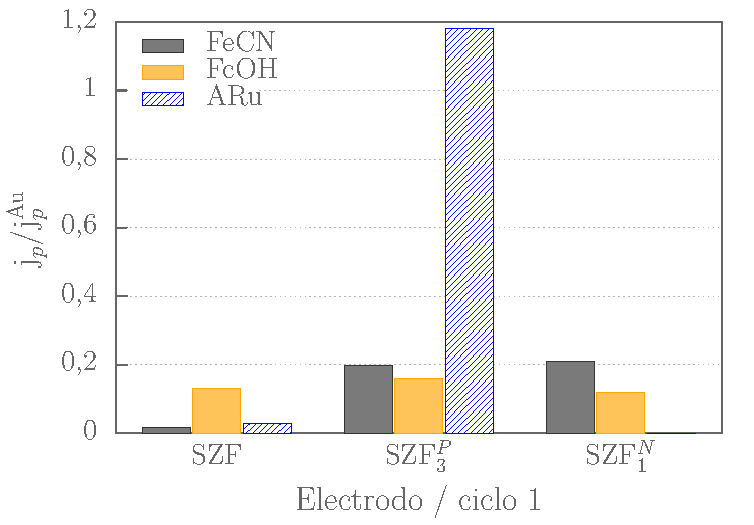
\includegraphics[trim=0 0 0 1cm,width=\textwidth]{Graficos/histogramas-ciclo1.pdf}
		 	  \end{subfigure}
		 	\begin{subfigure}[t]{0.495\textwidth}
		 	 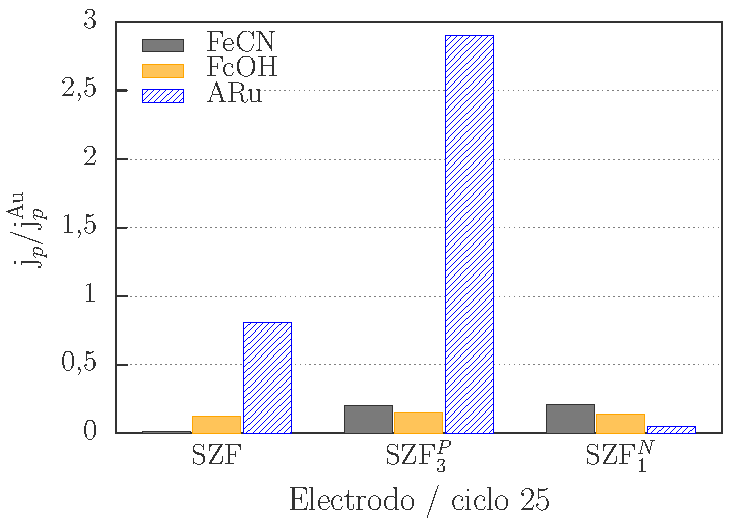
\includegraphics[trim=0 0 0 1cm,width=\textwidth]{Graficos/histogramas-ciclo25.pdf}
		 	  \end{subfigure}
			\begin{subfigure}[t]{0.495\textwidth}
		 	   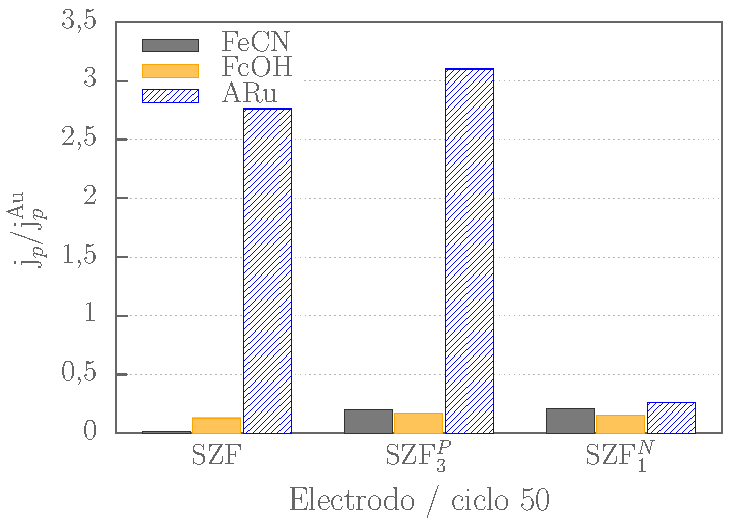
\includegraphics[width=\textwidth]{Graficos/histogramas-ciclo50.pdf}
		 	   \end{subfigure}
		      	\caption[Corriente de pico en distintos ciclos voltamperometricos]{Densidad de corriente anódica máxima en los ciclos 1, 25 y 50 para cada uno de los electrodos del sensor. Las sondas probadas fueron \fc \SI{1}{\milli\Molar}, \fe\space \SI{1}{\milli\Molar} y \ru\space \SI{1}{\milli\Molar} en KCl \SI{100}{\milli\Molar} a una velocidad de barrido de \SI{50}{\milli\volt\per\second}.}
		      	\label{fig:barras}
		      	\end{figure}
     	
	 Se puede ampliar aún más el análisis anterior agregando otras variables para la identificación de los analitos, tales como el potencial formal medio de cada sonda ($E^{\circ}$) y la separación de potenciales entre los picos anódico y catódico ($\Delta E$). Estos dos valores son tomados directamente de los voltagramas correspondientes al electrodo de Au desnudo y permiten cuantificar dos variables electroquímicas propias de cada sonda comparables con bases de datos bibliográficas.
	
		\begin{figure}[b!]
			   	    \begin{subfigure}[t]{0.325\textwidth}
			        	\includegraphics[trim=1.1cm 0cm 2.2cm 0cm,width=\textwidth]{Graficos/radial-ru-ciclo1-2.pdf}
			        	%\vspace*{-0.40cm}\caption{\aminorutenio\space \SI{10}{\milli\Molar}.}
			         	%\label{fig:Ru10mM}
			     		\end{subfigure}
			   	    \begin{subfigure}[t]{0.325\textwidth}
			        	\includegraphics[trim=1.1cm 0cm 2.2cm 0cm,width=\textwidth]{Graficos/radial-ru-ciclo25-2.pdf}
			       		%\vspace*{-0.40cm}\caption{\aminorutenio\space \SI{6}{\milli\Molar}.}
			         	%\label{fig:Ru63mM}
			     		\end{subfigure}
		     		\begin{subfigure}[t]{0.325\textwidth}
			        	\includegraphics[trim=1.1cm 0cm 2.2cm 0cm,width=\textwidth]{Graficos/radial-ru-ciclo50-2.pdf}
			       		%\vspace*{-0.40cm}\caption{\aminorutenio\space \SI{3}{\milli\Molar}.}
			         	%\label{fig:Ru315mM}
			     		\end{subfigure}
		     		\begin{subfigure}[t]{0.325\textwidth}
			        	\includegraphics[trim=1.1cm 0cm 2.2cm 0cm,width=\textwidth]{Graficos/radial-fecn-ciclo1-2.pdf}
			       		%\vspace*{-0.40cm}\caption{\aminorutenio\space \SI{1.5}{\milli\Molar}.}
			         	%\label{fig:Ru1575M}
			     		\end{subfigure}
		 	   	   	\begin{subfigure}[t]{0.325\textwidth}
			        	\includegraphics[trim=1.1cm 0cm 2.2cm 0cm,width=\textwidth]{Graficos/radial-fecn-ciclo25-2.pdf}
			       		%\vspace*{-0.40cm}\caption{\aminorutenio\space \SI{0.6}{\milli\Molar}.}
			         	%\label{fig:Ru063mM}
			     		\end{subfigure}
		     		\begin{subfigure}[t]{0.325\textwidth}
			        	\includegraphics[trim=1.1cm 0cm 2.1cm 0cm,width=\textwidth]{Graficos/radial-fecn-ciclo50-2.pdf}
			       		%\vspace*{-0.40cm}\caption{\aminorutenio\space \SI{0.3}{\milli\Molar}.}
			         	%\label{fig:Ru0315mM}
			     		\end{subfigure}
			     	\begin{subfigure}[t]{0.325\textwidth}
			        	\includegraphics[trim=1.1cm 0cm 2.2cm 0cm,width=\textwidth]{Graficos/radial-fcoh-ciclo1-2.pdf}
			       		%\vspace*{-0.40cm}\caption{\aminorutenio\space \SI{60}{\micro\Molar}.}
			         	%\label{fig:Ru0063mM}
			     		\end{subfigure}
		     		\begin{subfigure}[t]{0.325\textwidth}
			        	\includegraphics[trim=1.1cm 0cm 2.2cm 0cm,width=\textwidth]{Graficos/radial-fcoh-ciclo25-2.pdf}
			       		%\vspace*{-0.40cm}\caption{\aminorutenio\space \SI{30}{\micro\Molar}.}
			         	%\label{fig:Ru00315mM}
			     		\end{subfigure}
		     		\begin{subfigure}[t]{0.325\textwidth}
			        	\includegraphics[trim=1.1cm 0cm 2.2cm 0cm,width=\textwidth]{Graficos/radial-fcoh-ciclo50-2.pdf}
			       		%\vspace*{-0.40cm}\caption{\aminorutenio\space \SI{15}{\micro\Molar}.}
			         	%\label{fig:Ru001575mM}
			     		\end{subfigure}	
			     	\caption{Marcas sensoriales para \ru, \fe\space y \fc\space para los ciclos electroquímicos 1, 25 y 50. Cabe destacar que para las sondas neutra y negativa (\fc\space y \fe) la marca permanece constante a lo largo de los ciclos. Para la sonda positiva (\ru) la marca va mudando en función de las propiedades permeoselectivas de cada electrodo del multisensor. Notar el cambio de escala para \ru\space en los electrodos \pdmZ\space y \pdmZ$^P_3$\space debido a la alta capacidad preconcentradora de estas películas para la sonda de carga positiva.} 
		     		\label{fig:radiales}
		      	   	\end{figure}
		
		 Para poder representar conjuntamente todas estas variables se ha recurrido a gráficos radiales (figura \ref{fig:radiales}), ya que son variables con distintas unidades y escalas asociadas. Los valores representados fueron distribuidos a lo largo de cinco ejes: densidad de corriente normalizada ($\text{j}_p/\text{j}_p^\text{Au}$) para los electrodos \pdmZ, \pdmZ$^P_3$, \pdmZ$^N_1$, diferencia entre el potencial anódico y catódico ($\Delta E$) y potencia formal medio ($E^{\circ}$) de cada sonda. Estos gráficos permiten visualizar rápidamente tanto información termodinámica como cinética. El área especifica, o marca sensorial, que queda delimitada para los gráficos de las sondas \fc\space y \fe, permanece inalterable de ciclo en ciclo, indicando un estado de equilibrio desde el primer ciclo para ambos analitos. También se observa que para \fe\space la señal es nula en \pdmZ\space debido a una fuerte repulsión electrostática determinada por la carga negativa de la película, mientras que para el \fc, sonda de carga neutra, la densidad de corrientes para los tres recubrimientos (\pdmZ, \pdmZ$^P_3$, \pdmZ$^N_1$) es prácticamente idéntica, sugiriendo una interacción electrostática prácticamente nula con las distintas películas delgadas mesoporosas. El área para la sonda positiva evoluciona con los sucesivos ciclos debido a la cinética de adsorción, incluyendo el tiempo como un parámetro más que se suma para construir la marca sensorial. 

		 Estos experimentos, sobre la base de un multisensor, muestran el gran potencial de los dispositivos para identificar y cuantificar analitos electroactivos o discriminar entre grupos de compuestos generando marcas sensoriales para cada uno de ellos. 
					     
\section{Conclusiones}

	Se presentaron en este capítulo los resultados obtenidos durante el proceso de fabricación de los multisensores. Se idearon dos diseños, de los cuales el segundo (retroalimentado de la experiencia del primero) es más compacto, incorpora más electrodos por multisensor y prevé el uso de contraelectrodo y pseudoreferencia integrados en el mismo dispositivo.
	
	Los mismos fueron fabricados por un conjunto de técnicas conocidas como \textit{top-down}, propios de la microelectrónica como: fotolitografía óptica, deposición por pulverización catódica y \textit{lift-off}, entre otras. Se establecieron las condiciones óptimas de proceso para cada etapa, y, una vez conseguido resultados satisfactorios para la fabricación, se evaluó el desempeño electroquímico de los sensores, el cual resulto excelente. Los resultados obtenidos en la caracterización de los mismos fueron presentados en la sección \ref{sec:respuesta_sondas_au}, pág. \pageref{sec:respuesta_sondas_au}. 

	Sobre los electrodos de (Ti,Cr)\textbar Au se realizaron los primeros depósitos de películas delgadas mesoporosas de sílice. En esta etapa surgieron algunas dificultades, en particular, en lo referente al sensado electroquímico. Se realizó un estudio meticuloso en el cual se discutió cómo se afectó el desempeño electroquímico luego de los procesos de calcinación. Se llegó a la conclusión de que se ve impedida sensiblemente la transferencia de carga entre la sonda y el electrodo debido a fenómenos de difusión de interferencias hacia la superficie de los electrodos, y por lo tanto, también disminuye la calidad analítica de los multisensores.

	Éste fue el motivo principal para el desarrollo de procesos de síntesis de películas mesoporosas de SiO$_2$ a temperaturas menores que las clásicas de calcinación. Tiene como enormes ventajas minimizar los procesos difusivos y no recurrir a metales de ultra pureza, reduciendo sensiblemente los costos de los sensores. Las consecuencias directas del desarrollo fueron que se logró depositar óxidos sobre Au metalúrgico (Au3N) sin perder desempeño analítico y, a su vez, permitió depositar las \pdm\space sobre sustratos que sean estables a \SI{130}{\celsius}. Dicho desarrollo se estudia extensamente en el capítulo \ref{chap:Mesoporosos}, mientras que en el capítulo \ref{chap:Electroquimica} se estudia la estabilidad química y mecánica de la películas resultantes. Por otra parte el tratamientos a baja temperatura permite integrar la plataforma mesoporosa a una mayor variedad de electrodos, incluso utilizar sustratos poliméricos o térmicamente lábiles.

	Ya con el proceso de síntesis optimizado se escogieron las películas más estables para la fabricación de un multisensor prototipo. Se fabricaron nuevamente electrodos con el diseño <<calesita>> y se depositaron sobre ellas películas mesoporosas de Si$_{0.9}$Zr$_{0.1}$O$_2$ mediante el método de alto vacío. Sobre un multisensor se funcionalizaron localmente estás películas porosas con dihexadecilfosfato (DHDP) y 3-aminopropil trietoxisilano (APTES), específicamente sobre el área de dos electrodos, uno por cada funcionalización.
	
	Se analizaron las respuestas electroquímica de cada electrodo de este multisensor en función del ciclado electroquímico, obteniéndose patrones de respuesta para cada una de las sondas en función de la interacción entre la sonda y la película. Con el propósito de obtener una identificación inequívoca para cada sonda se amplió el análisis multivariable agregando dos variables más al sistema de datos: la diferencia entre el potencial de pico anódico y catódico y el potencial formal de cada sonda. De esta forma se confeccionaron gráficos radiales en función de la cantidad de ciclos electroquímicos con los valores para cada sonda, generando una marca sensorial cuantificable para cada uno de los analitos estudiados.





	